\documentclass[border=10pt]{standalone}
\usepackage{tikz}
\usepackage{amsmath}

\definecolor{inFill}{RGB}{183,224,177}
\definecolor{inLine}{RGB}{32,102,32}
\definecolor{hidFill}{RGB}{199,203,243}
\definecolor{hidLine}{RGB}{52,58,143}

\begin{document}
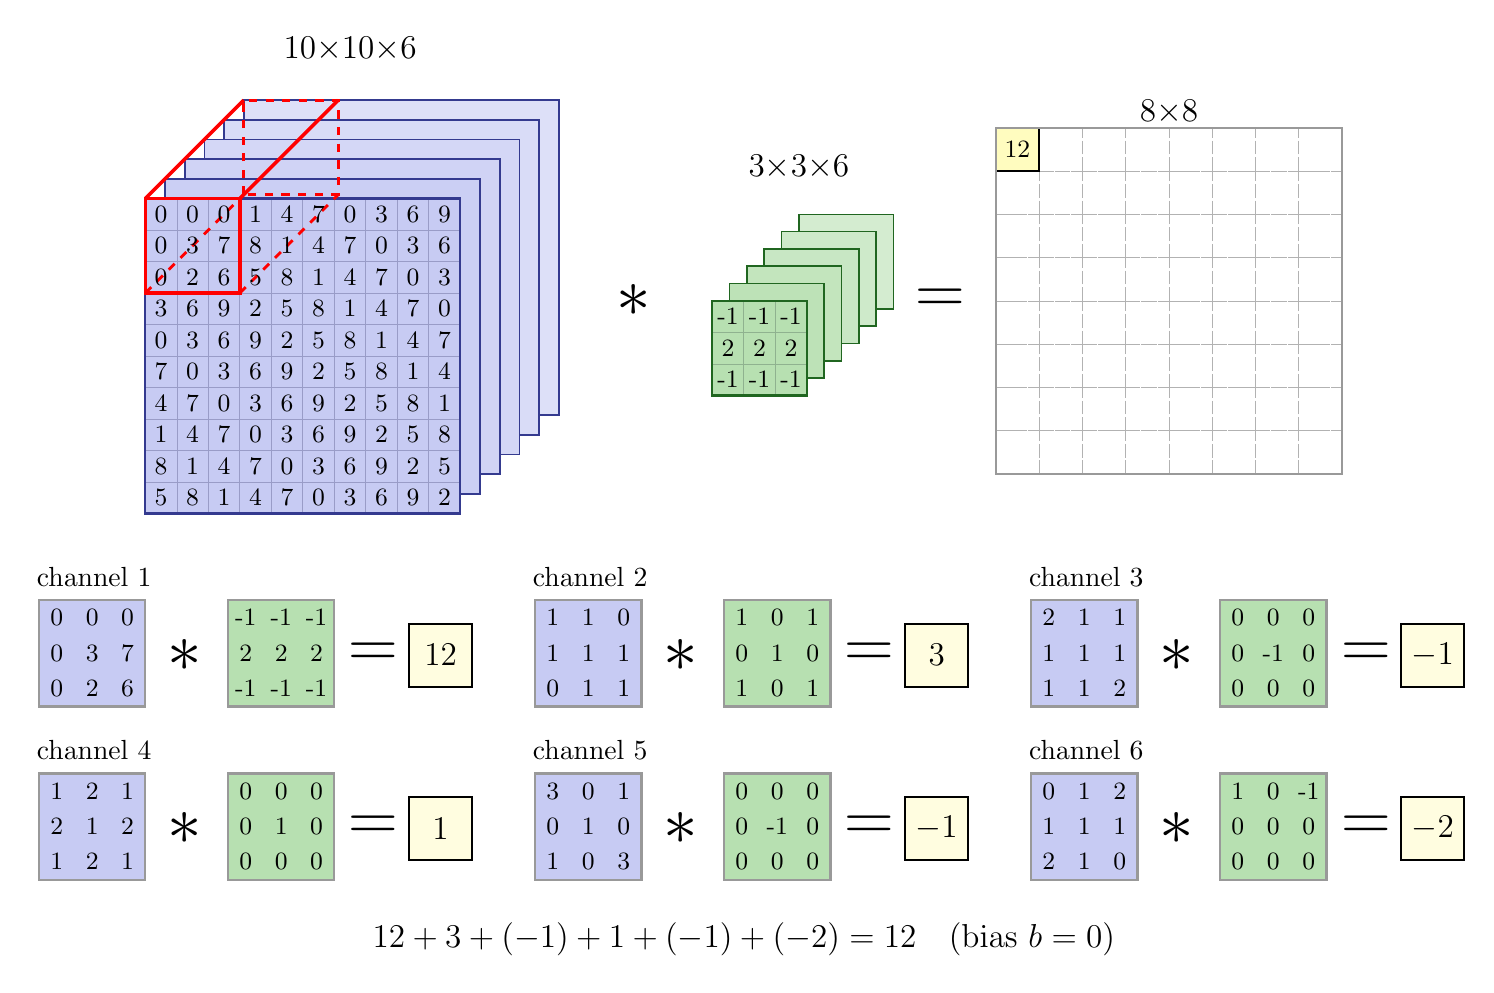
\begin{tikzpicture}[line width=0.8pt, font=\large]

  % ========== 特征图堆 10x10x6（淡紫）==========
  \newcommand{\fmstack}[2]{%
    \foreach \k in {5,4,...,0}{%
      \pgfmathtruncatemacro{\op}{100-8*\k}
      \fill[hidFill!\op, draw=hidLine, line width=0.6pt]
        ({#1+0.25*\k},{#2+0.25*\k}) rectangle ++(4,4);
    }
    \draw[hidLine!50, line width=0.25pt, shift={(#1,#2)}, step=0.4] (0,0) grid (4,4);
    \draw[hidLine] (#1,#2) rectangle ++(4,4);
  }

  % ========== 核堆 3x3x6（淡绿）==========
  \newcommand{\kstack}[2]{%
    \foreach \k in {5,4,...,0}{%
      \pgfmathtruncatemacro{\op}{100-8*\k}
      \fill[inFill!\op, draw=inLine, line width=0.6pt]
        ({#1+0.22*\k},{#2+0.22*\k}) rectangle ++(1.2,1.2);
    }
    \draw[inLine!50, line width=0.25pt, shift={(#1,#2)}, step=0.4] (0,0) grid (1.2,1.2);
    \draw[inLine] (#1,#2) rectangle ++(1.2,1.2);
  }

  % ========== 8x8 输出（左上角高亮 12）==========
  \newcommand{\resgrid}[2]{%
    \foreach \r in {0,...,7} \foreach \c in {0,...,7}
      \draw[gray!60, dashed, line width=0.3pt]
        ({#1+0.55*\c},{#2+0.55*\r}) rectangle ++(0.55,0.55);
    \fill[yellow!25] (#1,{#2+3.85}) rectangle ++(0.55,0.55);
    \node[font=\small] at ({#1+0.275},{#2+4.125}) {12};
    \draw[line width=0.6pt] (#1,{#2+3.85}) rectangle ++(0.55,0.55);
    \draw[gray!80] (#1,#2) rectangle ++(4.4,4.4);
  }

  % ========== 3x3 数值矩阵（#3=填充色）==========
  \newcommand{\mat}[4]{%
    \foreach \v [count=\m] in {#4} {%
      \pgfmathtruncatemacro{\c}{mod(\m-1,3)}
      \pgfmathtruncatemacro{\r}{div(\m-1,3)}
      \fill[#3] ({#1+0.45*\c},{#2+0.45*(2-\r)}) rectangle ++(0.45,0.45);
      \node[font=\small] at ({#1+0.45*\c+0.225},{#2+0.45*(2-\r)+0.225}) {\v};
    }
    \draw[gray!80] (#1,#2) rectangle ++(1.35,1.35);
  }

  \def\inpA{{0,0,0,0,3,7,0,2,6}}          % channel 1 的输入
  \def\kerA{{-1,-1,-1,2,2,2,-1,-1,-1}}    % channel 1 的核

  % ================= 顶行：体积卷积（整体右移居中）=================
  \begin{scope}[xshift=2.05cm]
    \fmstack{0}{-2}

    % ---- 红框：可见棱用实线（前面框 + 顶面两条连接棱）----
    \draw[red, line width=1.3pt] (0,0.8) rectangle ++(1.2,1.2);
    \draw[red, line width=1.3pt] (0,2.0) -- (1.25,3.25);
    \draw[red, line width=1.3pt] (1.2,2.0) -- (2.45,3.25);
    % ---- 红框：不可见棱用虚线（后面框一整圈 + 下方两条连接棱）----
    \draw[red, dashed, line width=1.0pt] (1.25,2.05) rectangle ++(1.2,1.2);
    \draw[red, dashed, line width=1.0pt] (0,0.8) -- (1.25,2.05);
    \draw[red, dashed, line width=1.0pt] (1.2,0.8) -- (2.45,2.05);

    % ---- 第一层（正面）数字：左上3x3=channel1，其余随意 ----
    \foreach \r in {0,...,9}{%
      \foreach \c in {0,...,9}{%
        \pgfmathtruncatemacro{\isc}{(\r<3 && \c<3) ? 1 : 0}%
        \ifnum\isc=1
          \pgfmathtruncatemacro{\val}{\inpA[\r*3+\c]}%
          \node[font=\small] at ({0.4*\c+0.2},{1.8-0.4*\r}) {\val};%
        \else
          \pgfmathtruncatemacro{\val}{mod(7*\r+3*\c+2,10)}%
          \node[font=\small] at ({0.4*\c+0.2},{1.8-0.4*\r}) {\val};%
        \fi
      }%
    }
    \node at (2.6,3.9) {10$\times$10$\times$6};

    \node[font=\Huge] at (6.2,0.7) {$\ast$};

    \kstack{7.2}{-0.5}
    % ---- 核第一层（正面）数字 = channel 1 的核 ----
    \foreach \r in {0,1,2}{%
      \foreach \c in {0,1,2}{%
        \pgfmathtruncatemacro{\val}{\kerA[\r*3+\c]}%
        \node[font=\small] at ({7.4+0.4*\c},{0.5-0.4*\r}) {\val};%
      }%
    }
    \node at (8.3,2.4) {3$\times$3$\times$6};

    \node[font=\Huge] at (10.1,0.7) {$=$};
    \resgrid{10.8}{-1.5}
    \node at (13,3.1) {8$\times$8};
  \end{scope}

  % ================= 下面：六个通道（垂直间距压缩）=================
  % ---- channel 1 ----
  \node[font=\normalsize] at (1.4,-2.8) {channel 1};
  \mat{0.7}{-4.45}{hidFill}{0,0,0, 0,3,7, 0,2,6}
  \node[font=\Huge] at (2.55,-3.8) {$\ast$};
  \mat{3.1}{-4.45}{inFill}{-1,-1,-1, 2,2,2, -1,-1,-1}
  \node[font=\Huge] at (4.95,-3.8) {$=$};
  \node[draw, thick, fill=yellow!12, minimum size=0.8cm] at (5.8,-3.8) {$12$};

  % ---- channel 2 ----
  \node[font=\normalsize] at (7.7,-2.8) {channel 2};
  \mat{7.0}{-4.45}{hidFill}{1,1,0, 1,1,1, 0,1,1}
  \node[font=\Huge] at (8.85,-3.8) {$\ast$};
  \mat{9.4}{-4.45}{inFill}{1,0,1, 0,1,0, 1,0,1}
  \node[font=\Huge] at (11.25,-3.8) {$=$};
  \node[draw, thick, fill=yellow!12, minimum size=0.8cm] at (12.1,-3.8) {$3$};

  % ---- channel 3 ----
  \node[font=\normalsize] at (14.0,-2.8) {channel 3};
  \mat{13.3}{-4.45}{hidFill}{2,1,1, 1,1,1, 1,1,2}
  \node[font=\Huge] at (15.15,-3.8) {$\ast$};
  \mat{15.7}{-4.45}{inFill}{0,0,0, 0,-1,0, 0,0,0}
  \node[font=\Huge] at (17.55,-3.8) {$=$};
  \node[draw, thick, fill=yellow!12, minimum size=0.8cm] at (18.4,-3.8) {$-1$};

  % ---- channel 4 ----
  \node[font=\normalsize] at (1.4,-5.0) {channel 4};
  \mat{0.7}{-6.65}{hidFill}{1,2,1, 2,1,2, 1,2,1}
  \node[font=\Huge] at (2.55,-6.0) {$\ast$};
  \mat{3.1}{-6.65}{inFill}{0,0,0, 0,1,0, 0,0,0}
  \node[font=\Huge] at (4.95,-6.0) {$=$};
  \node[draw, thick, fill=yellow!12, minimum size=0.8cm] at (5.8,-6.0) {$1$};

  % ---- channel 5 ----
  \node[font=\normalsize] at (7.7,-5.0) {channel 5};
  \mat{7.0}{-6.65}{hidFill}{3,0,1, 0,1,0, 1,0,3}
  \node[font=\Huge] at (8.85,-6.0) {$\ast$};
  \mat{9.4}{-6.65}{inFill}{0,0,0, 0,-1,0, 0,0,0}
  \node[font=\Huge] at (11.25,-6.0) {$=$};
  \node[draw, thick, fill=yellow!12, minimum size=0.8cm] at (12.1,-6.0) {$-1$};

  % ---- channel 6 ----
  \node[font=\normalsize] at (14.0,-5.0) {channel 6};
  \mat{13.3}{-6.65}{hidFill}{0,1,2, 1,1,1, 2,1,0}
  \node[font=\Huge] at (15.15,-6.0) {$\ast$};
  \mat{15.7}{-6.65}{inFill}{1,0,-1, 0,0,0, 0,0,0}
  \node[font=\Huge] at (17.55,-6.0) {$=$};
  \node[draw, thick, fill=yellow!12, minimum size=0.8cm] at (18.4,-6.0) {$-2$};

  % ---- 求和 ----
  \node at (9.65,-7.4)
    {$12+3+(-1)+1+(-1)+(-2)=12 \quad (\text{bias } b=0)$};
\end{tikzpicture}
\end{document}